% note: model paper 20 pages, Annaert et al, Long-run stock returns: evidence from Belgium 1838-2010

% using Elseveir template per https://www.elsevier.com/authors/author-schemas/latex-instructions
\documentclass[review]{elsarticle}

\usepackage{lineno,hyperref}
\modulolinenumbers[5]

\journal{Journal of \LaTeX\ Templates}
\bibliographystyle{elsarticle-num}

\usepackage{booktabs}
\usepackage{graphicx}
\graphicspath{{../alt-ed-survey/figures-and-tables}}
\usepackage{hyperref}
\usepackage{threeparttable}  
\usepackage{tikz}
\usetikzlibrary{calc,matrix}

\begin{document}
\begin{frontmatter}

\title{
    New Digital Education as the Market Solution to the Student Debt Crisis
    \tnoteref{titlenotes}
}

% \tnotetext[titlenotes]{
%     Go to \url{https://github.com/Vandivier/research-dissertation-case-for-alt-ed/tree/master/papers/student-debt-history}
%     to obtain source materials for this paper.
% }

\author[mymainaddress]{John Vandivier}
\address[mymainaddress]{4400 University Dr, Fairfax, VA 22030}
\ead{jvandivi@masonlive.gmu.edu}

\begin{abstract}
    I investigate social interest, or hype, in online learning.
    The two datasets of interest are derived from public search engine data for the United States over the period 2000-2020.
    This data is assessed for hype cycle dynamics.
    I find that interest in online learning and massive online open courses follow well-defined hype cycles.
    Interest in online learning has recovered from a low point.
    This indicates economic durability and positive growth outlook from an institutional point of view.
    I describe the history of online education as proceeding in three ages.
    New Digital Education is an affordable, employer-lead, hybrid learning approach to accredited higher education.
    New Digital Education emerges during the Second Age, from 2012-2017, and is normalized in the Third Age, from 2018 through the present.
    New Digital Education constitutes a sustainable market solution to the student debt crisis.
    A market solution to the student debt crisis undercuts the need for policy action.
\end{abstract}

\begin{keyword}
education economics, debt crisis, digital education, hype cycle, online learning, mooc
\MSC[2010] I20, I23, I28, N32
\end{keyword}

\end{frontmatter}

\pagebreak
\linenumbers
        
    \section{Introduction}

    Van Dusen discusses The Coming Crisis in Student Aid as early as 1979\cite{van1979coming}.
    Discussion on the issue has proceeded continuously.
    Forbes\cite{friedman2019student} noted that "Student loan debt in 2019 is the highest ever,"
    months before Ryan Craig would announce the Third Age of Online Education had begun\cite{craig2019welcome}.
    The fact of increasing debt in part casts doubt on the value proposition of online education.
    This paper contributes to the literature by mapping online education to the hype cycle, in addition to empirical and qualitative analysis.
    It turns out that cutting edge digital education is substantively different than the state of the art even a decade ago.
    This has implications for forecasting, policy, and the use of prior research.

    \section{Historical context}

    Ryan Craig argues that online learning has proceeded in three ages, beginning in the year 2000.
    I agree with his analysis,
    and in this section I review additional reasons selecting the same dates.
    Prior to the year 2000,
    the Institute for Higher Education Policy and Lumina Foundation provide further context
    on the origin of the student debt crisis\cite{foundation_2017}.
    
    The First Age runs from about 2000 to 2012.
    Craig argues that this is the age of the for-profit online university.
    I note three other reasons that the year 2000 is a reasonable date.
    In 2000, 55 percent of two and four year institutions offered distance education\cite{tabs2003distance}.
    This is the first year where most institutions offered distanced education.
    In 1997, 44 percent of institutions offered distance education\cite{sikora2002profile}.

    Secondly, 2000 begins the dot-com bust, which would last through 2002\cite{wollscheid2012rise}.
    From a hype cycle perspective, the bust is a trough of disillusionment.
    To survive the bust indicates economic durability, institutional fitness, and a positive continued growth outlook.
    Thirdly, NCES notes that a nontrivial 8 percent of students took at least one online course in 2000\cite{radford2011learning}.
    The figure increased to 20 percent by 2008.
    One might argue for beginning at the founding of Western Governors University in 1997, or after the end of the dot-com bust in 2002, but all of these plausible dates round to 2000.
    Ferrer gives an interesting history of what might be called the Zeroth Age of Online Education, exploring the developmental phase of remote learning prior to the turn of the millennium\cite{ferrer_2019}.

    Craig argues that a second age dominated by quasi-for-profits and online program managers (OPMs) began in 2012.
    It is important to note that the Massive Online Open Course (MOOC) era is realized roughly contemporaneously.
    Studying the cases of Khan Academy and Udacity is illustrative.
    In 2008, Clayton Christiansen and Michael Horn applied the theory of disruption to digital education\cite{horn2008disrupting}.
    Khan Academy was founded the same year\cite{tucker_2018}.
    Dan Friedman\cite{friedman2014mooc} notes that Udacity rolled out classes in 2012, with Coursera and edX enrolling their first students the same year.
    MOOCs reported outcomes far weaker than expected through 2013 and 2014, but recovery and continued innovation proceeded quickly.
    Uber was founded in 2009 and Facebook went public in 2012.
    These changes highlight the ability of the Second Age to capture important shifts in society and the economy.
    The spread of social media enables previously unprecedented normalization of online life.
    The sharing economy improves the economy through innovative, digitally-empowered business models.

    In 2013, Udacity began offering courses for college credit with San Jose State University\cite{shen_2015}.
    In 2014, Udacity entered into its first full-fledged program partnership with a university.
    Georgia Institute of Technology and Udacity announced an online Masters Degree in Computer Science for \$7000.
    This was 80 percent less than the on-campus equivalent\cite{onink2013georgia}.
    The same year, Udacity released its first signature alternative credential, the Nanodegree.

    A blended learning solution called Udacity Connect was piloted in 2016 and expanded in 2017.
    Udacity Connect's pilot achieved a 76 percent completion rate\cite{shah_2018}.
    As of 2019, Sebastian Thrun reports 4 percent is the MOOC completion rate,
    but Nanodegree programs have a 34 percent graduation rate, and using new personalized mentorship programs, cohorts commonly exceed 60 percent graduation rates.

    In 2016, Khan Academy applied for the \$100 million dollar grant
    by 100\&Change in order to create a globally recognized secondary education diploma.
    1,904 organizations applied for the grant\cite{conrad_2016}.

    
    When decisions were rendered in 2017, Khan Academy's proposal earned an honorable mention as one of the top ten in the education category,
    but it did not earn a financial award\cite{cushing_2017}.

    Like Udacity, Khan Academy is an online learning provider which went through a period of immense excitement followed by failure,
    and also like Udacity, Khan Academy achieved a remarkable success on a different project during the same calander year as their disenchanting loss.
    In 2017, Khan Academy released the results of a study they conducted with the College Board.
    It showed that studying for the SAT using Khan Academy is associated with 115-point average score increase\cite{khan_academy_sat_2017}.
    Khan Academy became the official practice partner for AP exams in 2017\cite{khan_academy_partner_2017}.

    Not only do Udacity and Khan Academy share a Jungian hero typology,
    they have both evolved from traditional learning competitors to traditional learning allies
    Like Coursera, edX, and others, the best-of-breed alternative learning providers of today are not substituting for traditional education providers,
    they are integrating with them. Likewise, the best-of-breed traditional providers are not rejecting new learning approaches,
    they are partnering with them, awarding credit to students for alternative learning, and even supplying online education providers with content.

    Summarily, there are three important changes which occur in the Second Age of Online Education, which I date from 2012-2017, in addition to the proliferation of OPMs.
    First, the MOOC revolution occurs through digitally-native, non-accredited online learning providers.
    Second, digitally-native learning providers go through a hero's journey.
    Providers like Coursera and Udacity initially fail to meet expectations, then improving outcomes significantly in a short period.
    Third, the education market integrates and equilibrates to some degree.
    Hybridization becomes a new normal.
    This hybrid norm is true of the industry leaders, but it will be explored quantitatively in the subsequent section on data.
    Traditional providers are brought online, and digitally native organizations begin exploring offline education.

    The Third Age of Online Education is characterized by affordable college, driven by employer financing.
    It has also been characterized as an age of MOOC-based degrees.
    In 2013, SHRM reported that 61 percent of employers offer tuition assistance\cite{cherry2014rejuvenating}.
    In 2017, World at Work found that 85 percent of employers offered such a benefit,
    with another 7 percent offering non-reimbursement tuition assistance, such as upfront tuition discounts\cite{talentculture_2018}.
    In 2019, reimbursement was negligibly higher with an offering at 86 percent of employers\cite{worldatwork_2019}.
    This increase in tuition assistance is invigorated in part by the emergence of a new kind of employee benefit intermediary,
    often partnering with online education providers.

    Guild Education is an example of this new kind of benefits intermediary. Walmart is the largest employer in the United States.
    Walmart and Guild partnered to provide higher education to Walmart employees, including part-time employees, forming an interesting case study.
    Walmart's program began in 2018 and provides college education for one dollar per day\cite{walmart_2018}.
    As of January 2020, Walmart's program allows access to around 40 degrees through about half a dozen online providers\cite{guild_walmart_2020}.
    Providers include the University of Florida and Southern New Hampshire University.
    Walmart's education benefit also provides a high school completion program and free ACT and SAT preparation assistance.

    Employers are motivated to provide this service because they generate return through such vectors as improved employee retention.
    Guild clients see 120 to 210 percent return to education spend\cite{hunter_2019}.
    This is consistent with the 129 percent return observed by Accenture and the Lumina Foundation,
    who published return to education spend informatino for Cigna's education reimbursement program\cite{mccann_2016}.

    While online learning has become normal, perception as normal lags slightly behind.
    Surveys from 2017 and 2018 show that students, employers, and the general public generally believe
    an online degree is equal to or better than on-campus\cite{venable_2019}.
    The general public is the least positive of these three groups.
    While most employers support online learning,
    about 18 percent of students state that employer perception of an online degree is a concern.

    Taking advantage of employer-financed education presupposes working while learning.
    This turns out to also be an established norm in higher education.
    In 2015, a report from Georgetown University showed that more than 70 percent of college students
    worked while learning over the prior 25 years\cite{carnevale2015learning}.
    For most students the academic effects are not important,
    but they find an important academic threat to low-income working learners who work more than 15 hours each week.
    Darolia\cite{darolia2014working} introduces additional controls and concludes that working
    marginally increasing hours does not negatively affect grades, although it does slow credit accumulation.

    While hybridization began in the Second Age, it is fully in place throughout the Third Age.
    Class Central lists online courses and publishes related news.
    Dhawal Shah is a subject matter expert on MOOCs and online learning with Class Central.
    Shah identifies 2018 as the year of MOOC-based degrees, and notes that significant growth continues in 2019\cite{shah_2019}.

    \section{Data}

    I demonstrate hype cycles using two kinds of Google search data.
    The first is ordinary search volume and the second is Google Trends data.
    Both sources are intended to proxy social attention, or hype.
    There are several important caveats when using these sources.
    First, Google Trends data extends as far back as 2004,
    but this is too late to capture hype around the dot-com boom.
    Relatedly, Google News Archive Search became available in 2006.
    While Google retroactively added older news, I will shortly demonstrate serious coverage gaps with this information.
    As a result, general search data is used instead of media data in particular.

    A final caveat is that these search-based measures of hype ignore sentiment and focuses only on volume.
    Sentiment analysis of the underlying media coverage is quite feasible,
    but it is hardly necessary because it has been qualitatively covered in the section on historical context
    and also because the sustained growth in the market associated with hype already implies positive sentiment on average.

    Google Trends provides an index of search volume, called interest, over time.
    The interest index is not an exact search frequency.
    Interest takes a value between 0 and 100, inclusive, and is normalized across each concurrently measured series.
    The key result is the establishment of a hype cycle in the trend of a series in relation to itself over time.
    Google Trends data is available using Google-defined topics as well as keyword matching.
    Google-defined topics are generally preferred for precision, and that is the form of data which I use.
    Keyword matching is less precise because there is a boolean or statement used by the querying engine, resulting in many false positive results and significant noise in the data.
    With Google-defined topics, Google utilizes machine intelligence to ensure relevant, apples-to-apples results are contained in a trend signal.
    Western Governors University is a great example of why this distinction is important.
    As a keywords search, search volume would be reported for any search using any of those words.
    Irrelevant results for Western Union, Best Western, and University of Texas would all be included.
    Google Trends allows for location-based filtering, and the Unites States are selected as the scope of this study.
    
    Western Governors University was founded in 1997.
    Launching a well-funded organization like WGU is expected to generate hype.
    This provides an edge case which helps validate the quality of Google News data.
    Google News data is revaled to be problematic immediately when a search from January 1990 through December 2001 yields zero results.
    This concern is bolstered when it is revealed that a search for the word "water" results in only 81 results over the same time period.
    Further inspection shows that about 23 of the 81 results were actually published during the specified time period.
    
    In contrast with Google News data, an ordinary Google search for water, filtered to the dates 1990 through 2001, yield hundreds of results.
    A cursory look indicates that these web pages were in fact published during the specified date range.
    Searching for Western Governors University in the ordinary way presents with more than zero results.
    While ordinary Google search data has plenty of peculiarities, it seems preferred due to this preliminary validation.
    Google Trends data is preferred to ordinary search results, but the founding of WGU precedes available Google Trends data.
    Ordinary search result data is global in principle, but in practice the early search data on WGU is driven within the United States.

    \section{Results}

    The first main result is depicted in Figure \ref{fig:google_trends_digital_education}.
    In this graph we can see that online degrees have sustained high interest for as long as Google data has been available.
    That is, from 2004 to 2020, the present year.
    While general interest has remained high, there is a clear downturn in 2010, and a recovery of interest in 2017.
    MOOCs, in contrast, see a clear uptick in interest in 2012, and the beginning of decline the next year.
    The general interest in MOOCs never recovers.

    \begin{figure}[h!]
        \centering
        \caption{Annualized Interest}
    
        \begin{tikzpicture}[element/.style={minimum width=1cm, minimum height=0.75cm}]
        \node (n1) [above=0.25cm] {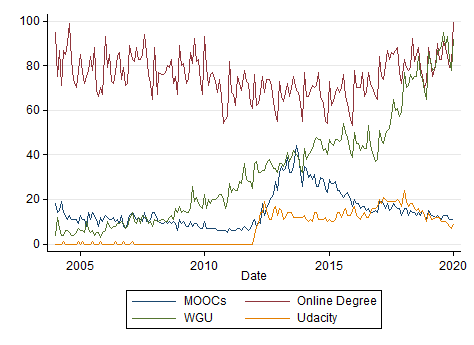
\includegraphics[width=1\textwidth]{./google-trends-digital-education.png}};
        \end{tikzpicture}

        \label{fig:google_trends_digital_education}
        \end{figure}

    The particular case of Udacity is slightly different compared to the general data on MOOCs,
    and the particular case of Western Governors University is different than the general trend in online degrees.
    Udacity sees a local maximum in June 2012, followed by decline.
    Udacity recovers to an even higher local maximum in January 2018.
    Interest in Udacity is presently declining, but Udacity has declined and recovered before,
    in contrast to the concave-down trend for MOOCs generally.
    This empirical data lines up well with the Three Ages conceptualization.

    In the Third Age, learning online is growing in interest, but it is being fueled by providers
    like WGU, rather than providers like Udacity.
    WGU presents an odd case here, because there is no substantive hype cycle.
    One might argue for a minor cycle from August 2015 to May 2017, but this pales in comparison to accelerating adoption across the whole period.
    On Google Trends data alone, it appears plausible that WGU's growth is manic and ripe for correction.

    The WGU mania theory has two issues.
    First, in the section on historical context, we uncovered fundamental changes in the economy which would stimulate growth in WGU interest in the Third Age.
    Namely, growth in employer tuition assistance, growing social desire for online learning,
    and the decline of for-profit providers like University of Phoenix.
    Secondly, the truncation of data in 2004 creates a bit of an illlusion.
    As we see in Figure \ref{fig:wgu_search_results}, 2004 was near a low point in WGU's history.
    The dot-com boom and bust is clearly depicted with WGU as a participant.
    Figure \ref{fig:wgu_search_results} is constructed utilizing Google's Advanced Search to filter results by year
    \footnote{
        Result count obtained using the boolean query "Western Governor's University" OR "Western Governors University" was used.
        Plenty of online discussion on WGU involves this typo.
        The count used excludes articles which Google excludes by default.
        Google excludes some web results by default, generally because the excluded results seem to be copies of results already shown.
    }.

    \begin{figure}[h!]
        \centering
        \caption{WGU Search Results by Year}
    
        \begin{tikzpicture}[element/.style={minimum width=1cm, minimum height=0.75cm}]
        \node (n1) [above=0.25cm] {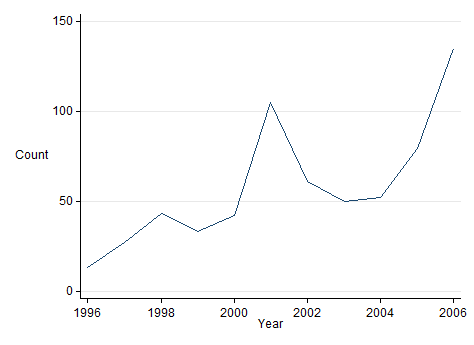
\includegraphics[width=1\textwidth]{./google-search-wgu.png}};
        \end{tikzpicture}

        \label{fig:wgu_search_results}
        \end{figure}
    
    \section{Conclusions}

    This paper demonstrates that interest in online degrees has survived the trough of disillusionment
    and is becoming a normal part of higher education.
    Renewed interest in online education has coevolved with changes in society and the character of
    online learning. Evidence supports a Three Ages description of the character of online education.
    Online enrollments increased in 2017, even while general postsecondary enrollment declined\cite{lederman2018online}.
    This indicates that not only is online education trending up, but it is substituting for traditional education.

    These findings have several implications. For policy, an implication is that existing policies
    including the write off for tuition reimbursement are sufficient.
    Because employers are financing employee education, the need for further education subsidy is undercut.
    For students, a strategy of learning while working is recommended,
    although questions remain about the best strategy for full-time workers with low income.

    For students, Third Age learning means a higher private return to education.
    Because this lifestyle is provisioned by an employer,
    the distinction between continuous professional education and undergraduate education blurs.

    For academics, the Three Ages characterization means that much prior research is now obsolete.
    In turn, demand for new research is stimulated.
    Hype cycle dynamics, aggregate market growth, and the research presented in this paper
    result in an expectation of continued growth in online education in the future.
    Continued social normalization and financial improvements are also expected,
    but many questions remain.

    The growth rate of student debt is expected to decrease, but the rate and schedule of this decrease isn't clear.
    Whether the growth rate will move close to zero or past zero into substantially negative territory isn't clear.
    It's clear that learners and employers generally support online education,
    but it's not clear why this general support is resisted by some.
    Microanalysis which accounts for employer and learner heterogeneity in the Third Age
    of online learning is needed to create insights which are optimally actionable for particular individuals.

    \bibliography{./BibFile}

    \end{document}
